\documentclass[a4paper,12pt]{article}
\setlength{\headheight}{68.803pt}
\addtolength{\topmargin}{-56.803pt}

\usepackage[utf8]{inputenc}
\usepackage[T1]{fontenc}
\usepackage{lmodern}
\usepackage[nopatch=footnote]{microtype}
\usepackage{fvextra}
\DefineVerbatimEnvironment{Verbatim}{Verbatim}{
  breaklines=true,
  breakanywhere=true,
  frame=single,
  fontsize=\small
}

% Impostazione dei margini con geometry
\usepackage[
  left=1in,
  right=1in,
  top=3cm,
  bottom=1in
]{geometry}

\usepackage[
    colorlinks=true,
    linkcolor=black,
    urlcolor=blue,
    citecolor=blue,
    pdfborder={0 0 0},
    pdfauthor={Massimo Mantineo},
    pdftitle={Socket UDP e TCP in C},
    pdfsubject={Laboratorio di Reti e Sistemi Distribuiti: HANDS-ON},
]{hyperref}

\usepackage{graphicx}
\graphicspath{{../../assets/}{../../assets/ho1/}{../../assets/ho2/}{../../assets/ho3/}{../../assets/ho4/}{../../assets/ho5/}{../../assets/ho6/}{../../assets/ho7/}{../../assets/ho8/}{../../assets/ho10/}}
\usepackage{tikz}
\usetikzlibrary{positioning, arrows.meta}
\usepackage{listings}
\usepackage{xcolor}
\usepackage{amsmath, amssymb}
\usepackage{fancyhdr}
\usepackage{setspace}
\usepackage{pgfplots}
\pgfplotsset{compat=1.17}
\usepackage{booktabs}
\usepackage[skins, listings]{tcolorbox}
\usepackage{float}

\newtcblisting{terminal}[1][]{
    listing only,
    colback=black!85!white,
    colframe=black!70!white,
    colupper=green!80!white,
    coltitle=white,
    title=#1,
    fonttitle=\bfseries\sffamily,
    listing options={
        language={},
        basicstyle=\ttfamily\small\color{green!80!white},
        backgroundcolor={},
        frame=none,
        breaklines=true,
        showstringspaces=false,
        numbers=none
    },
    enhanced,
    drop shadow,
    arc=3mm
}

\newtcblisting{ccode}[1][]{
    listing only,
    colback=blue!3!white,
    colframe=blue!70!black,
    title=#1,
    fonttitle=\bfseries\sffamily,
    listing options={
        style=cstyle,
        backgroundcolor={},
        frame=none
    },
    enhanced,
    drop shadow,
    arc=3mm
}

\setlength{\footskip}{50pt}

% Impostazioni per i listing del codice C
\lstdefinestyle{cstyle}{
    language=C,
    basicstyle=\ttfamily\small,
    numbers=left,
    numberstyle=\tiny,
    stepnumber=1,
    numbersep=5pt,
    backgroundcolor=\color{white},
    showspaces=false,
    showstringspaces=false,
    showtabs=false,
    frame=single,
    tabsize=4,
    captionpos=b,
    breaklines=true,
    breakatwhitespace=true,
    keywordstyle=\color{blue}\bfseries,
    commentstyle=\color{green!50!black},
    stringstyle=\color{red},
}
\lstset{style=cstyle}

% Impostazione di fancyhdr per header e footer
\pagestyle{fancy}
\fancyhf{}

\fancyhead[L]{%
  \parbox[b]{0.45\textwidth}{%
    \small
    Student Name: Massimo Mantineo\\
    Student ID: 541924
    \vspace{20pt}
  }%
}
\fancyhead[C]{%
  \parbox[b]{0.2\textwidth}{%
    \centering
    \normalsize \bfseries
    LabReSiD25\\
    Hands-On 1
    \vspace{20pt}
  }%
}
\fancyhead[R]{%
  \parbox[b]{0.35\textwidth}{%
    \flushright
    
\includegraphics[width=3.5cm]{logo_unime_orizontale.png}
    \vspace{15pt}
  }%
}

\renewcommand{\contentsname}{Indice}

\title{\vspace{-2cm}Report: Socket UDP e TCP in C\\
\large (Hands-On 1)}
\author{Massimo Mantineo \\ Matricola: 541924}
\date{MESSINA, A.A. 2024/2025}

\begin{document}

% Pagina di copertina
\begin{titlepage}
    \thispagestyle{empty}
    \centering
    \vspace*{1cm}
    
\includegraphics[width=6cm]{logo_unime_orizontale.png}\par\vspace{1cm}
    \vspace{2cm}
    {\Large \textbf{Università degli Studi di Messina}\par}
    {\large Dipartimento MIFT - Corso di Laurea Triennale in Informatica (L-31)\par}
    \vspace*{1cm}
    {\large Laboratorio di Reti e Sistemi Distribuiti\par}
    \vspace{1cm}
    {\Large \textbf{HANDS-ON 1:}\\
    Socket UDP e TCP\par}
    \vspace{2cm}
    {\large Massimo Mantineo \par}
    {\large Matricola: 541924 \par}
    \vfill
    {\large Messina, A.A. 2024/2025 \par}
\end{titlepage}

\clearpage
\pagestyle{fancy}
\tableofcontents
\newpage

\section{Problem Statement}
L'obiettivo di questa prima esercitazione (Hands-On 1) è l'acquisizione delle competenze fondamentali nella programmazione di rete tramite l'interfaccia dei \textbf{Berkeley Sockets}. La sfida consiste nel progettare e implementare due architetture client-server basilari per analizzare le divergenze operative tra i due protocolli dominanti del livello di trasporto: \textbf{TCP} (Transmission Control Protocol) e \textbf{UDP} (User Datagram Protocol). Le specifiche richiedono di validare l'affidabilità del flusso di byte nel TCP e la natura orientata ai datagrammi dell'UDP, ispezionando il comportamento del kernel tramite l'analisi dei file descriptor e del traffico di rete.

\section{Stato dell'Arte}
La comunicazione nei sistemi distribuiti si basa sulla suite di protocolli TCP/IP, dove il livello di trasporto offre diverse astrazioni di servizio.

L'interfaccia di programmazione utilizzata è quella dei \textbf{POSIX Sockets}, che astrae la risorsa di rete come un \textbf{File Descriptor (FD)}, permettendo l'uso di primitive di I/O standard del sistema operativo.

\section{Metodologia ed Implementazione}
La soluzione è stata articolata in due coppie di programmi C (Client/Server) che utilizzano le librerie \texttt{<sys/socket.h>} e \texttt{<arpa/inet.h>}. Lo sviluppo ha seguito una metodologia incrementale: configurazione del socket, binding locale e gestione del flusso dati.

\begin{figure}[H]
    \centering
    \begin{tikzpicture}[
        node distance=1.5cm,
        box/.style={rectangle, draw=blue!70, fill=blue!5, thick, minimum width=3cm, minimum height=1cm, align=center, font=\small\sffamily},
        arrow/.style={-Stealth, thick, blue!70}
    ]
        % Server Sides
        \node[box] (s_sock) {socket()};
        \node[box, below=0.8cm of s_sock] (s_bind) {bind()};
        \node[box, below=0.8cm of s_bind] (s_list) {listen()};
        \node[box, below=0.8cm of s_list] (s_acc) {accept()};
        \node[box, below=1.5cm of s_acc] (s_rw) {read/write};

        % Client Sides
        \node[box, right=4cm of s_sock] (c_sock) {socket()};
        \node[box, below=2.5cm of c_sock] (c_conn) {connect()};
        \node[box, below=1.5cm of c_conn] (c_rw) {write/read};

        % Connections
        \draw[arrow] (s_sock) -- (s_bind);
        \draw[arrow] (s_bind) -- (s_list);
        \draw[arrow] (s_list) -- (s_acc);
        \draw[arrow] (c_sock) -- (c_conn);
        \draw[arrow, dashed] (c_conn) -- node[above, font=\tiny, color=black] {TCP Handshake} (s_acc);
        \draw[arrow] (s_acc) -- (s_rw);
        \draw[arrow] (c_conn) -- (c_rw);
        \draw[arrow, <->, color=orange!80!black] (s_rw) -- node[above, font=\tiny] {Data Exchange} (c_rw);

        % Labels
        \node[above=0.2cm of s_sock, font=\bfseries] {SERVER (TCP)};
        \node[above=0.2cm of c_sock, font=\bfseries] {CLIENT (TCP)};
    \end{tikzpicture}
    \caption{Workflow di interazione tra Client e Server tramite Socket API.}
    \label{fig:socket_workflow}
\end{figure}

\subsection{Implementazione TCP: Byte Stream}
Il modello TCP adotta un approccio \textit{stateful}. Il server rimane in ascolto passivo (\texttt{listen}) finché non accetta (\texttt{accept}) una richiesta di connessione.
\begin{ccode}[Snippet Inizializzazione TCP]
int server_fd = socket(AF_INET, SOCK_STREAM, 0); // SOCK_STREAM per TCP
bind(server_fd, (struct sockaddr *)&address, sizeof(address));
listen(server_fd, 3);
int new_socket = accept(server_fd, (struct sockaddr *)&address, (socklen_t*)&addrlen);
\end{ccode}

\subsection{Implementazione UDP: Datagram Exchange}
Il modello UDP è \textit{stateless}. Viene creato un socket di tipo \texttt{SOCK\_DGRAM}, permettendo l'invio immediato tramite \texttt{sendto} e la ricezione con \texttt{recvfrom}, che restituisce contestualmente l'indirizzo del mittente per eventuali repliche.
\begin{ccode}[Snippet Inizializzazione UDP]
int sockfd = socket(AF_INET, SOCK_DGRAM, 0); // SOCK_DGRAM per UDP
bind(sockfd, (const struct sockaddr *)&servaddr, sizeof(servaddr));
recvfrom(sockfd, buffer, 1024, 0, (struct sockaddr *)&cliaddr, &len);
\end{ccode}


\subsection{Istruzioni di Esecuzione}
Per testare la comunicazione TCP e UDP, compilare i sorgenti con GCC:
\begin{terminal}[Build]
$ gcc server_tcp.c -o s_tcp
$ gcc client_tcp.c -o c_tcp
$ gcc server_udp.c -o s_udp
$ gcc client_udp.c -o c_udp
\end{terminal}

\section{Risultati}
La validazione del sistema è stata condotta su due fronti: l'analisi interna delle risorse di sistema e l'ispezione esterna del traffico.

\subsection{Analisi del File Descriptor}
Esaminando lo pseudo-filesystem \texttt{/proc}, è stato confermato che il kernel Linux assegna un intero (\texttt{FD 3}) per ogni socket creato, trattandolo come un file aperto. L'utility \texttt{lsof} ha validato il binding sulla porta 8080:
\begin{terminal}[Ispezione FD]
$ ls -l /proc/pid/fd
3 -> socket:[105681]
$ lsof -p pid | grep "UDP"
server_ud  3u  IPv4  UDP *:8080 
\end{terminal}

\subsection{Analisi Wireshark}
La cattura del traffico ha evidenziato graficamente il \textbf{Three-Way Handshake} (SYN, SYN-ACK, ACK) nel caso TCP, assente invece nello scambio UDP, confermando le differenze di overhead discusse in teoria.

\begin{figure}[H]
    \centering
    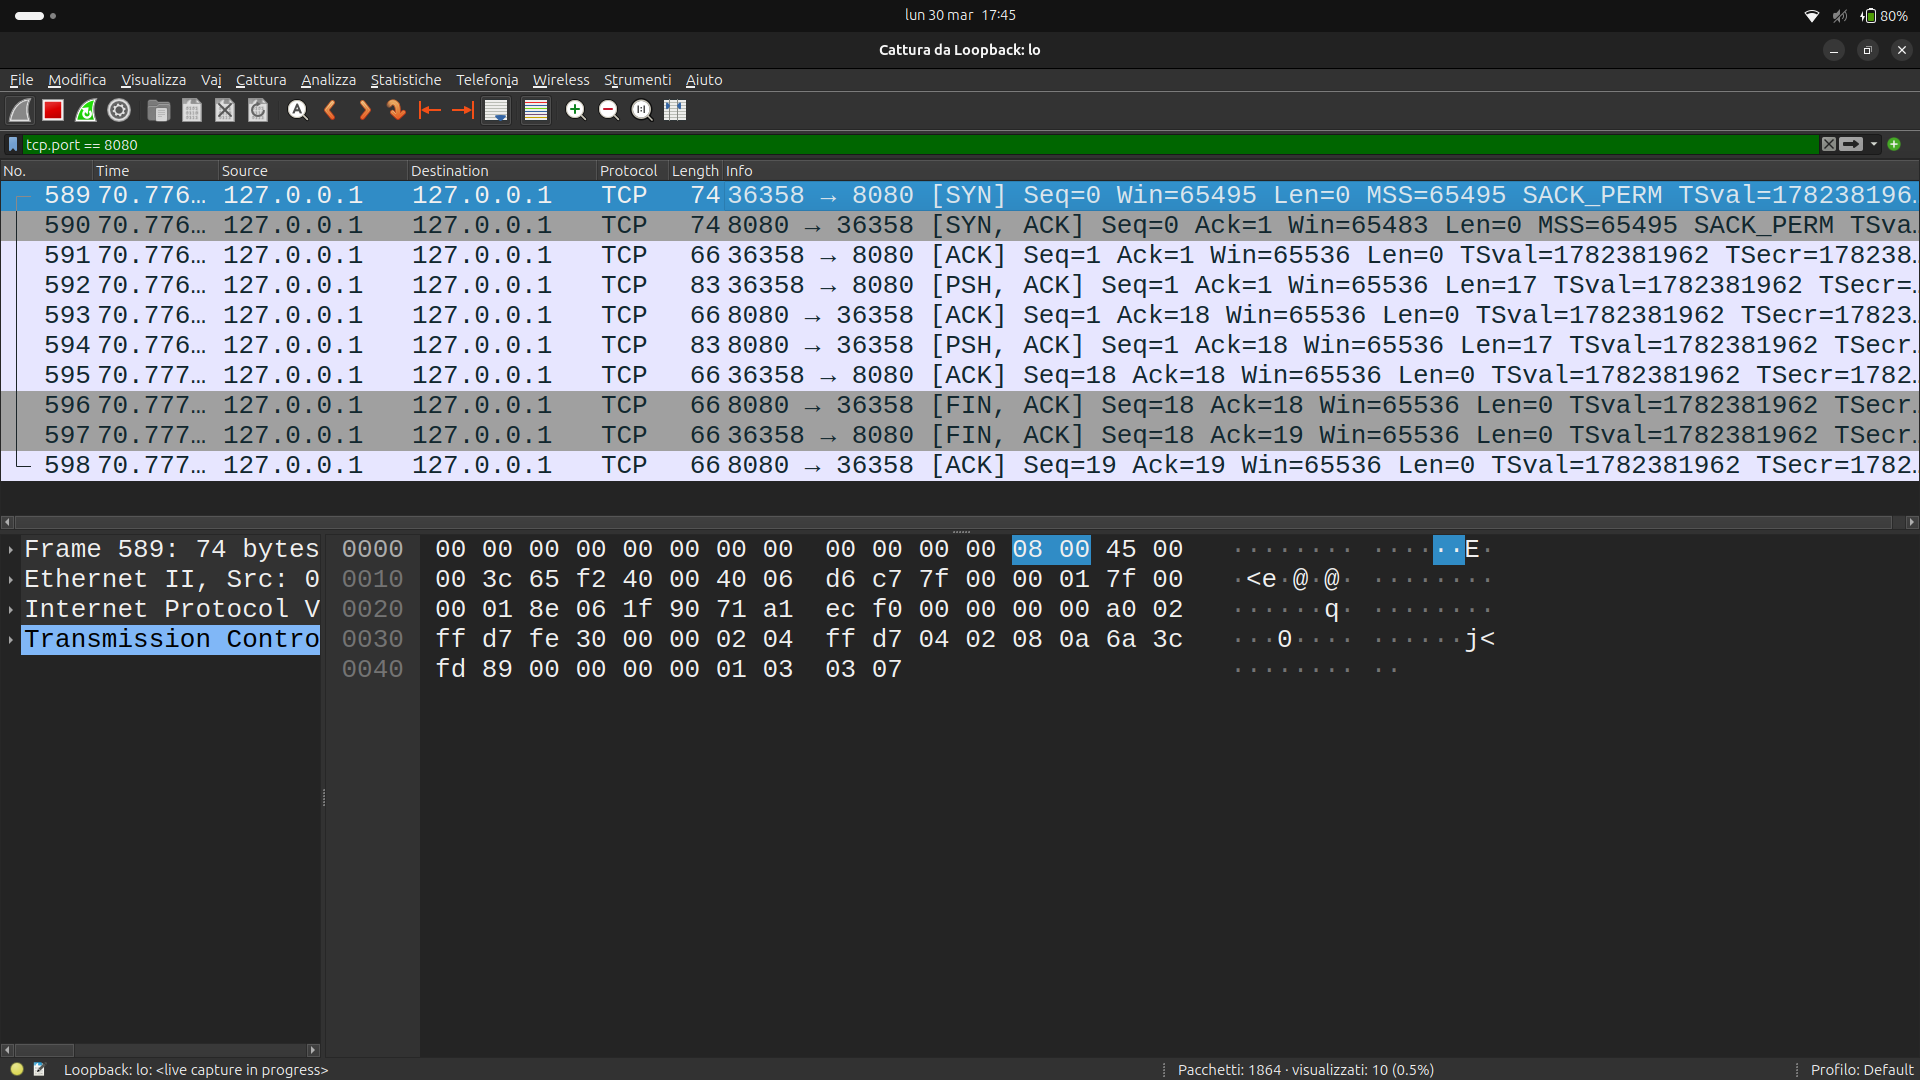
\includegraphics[width=0.85\textwidth]{ho1_wireshark_tcp.png}
    \caption{Handshake TCP e trasferimento dati catturati su loopback.}
\end{figure}

\section{Conclusioni e Sviluppi Futuri}
L'Hands-On 1 ha permesso di consolidare le basi della programmazione di rete e la comprensione della dualità tra affidabilità (TCP) ed efficienza (UDP). L'integrazione tra codice C e strumenti di diagnostica (Wireshark, lsof) ha fornito una visione \textit{full-stack} della comunicazione di rete.

\noindent \textbf{Sviluppi futuri:}
\begin{itemize}
    \item \textbf{Analisi Prestazionale}: Studio dell\'impatto della latenza di sistema sulla scalabilità dell\'architettura.
    \item \textbf{Ottimizzazione delle Risorse}: Refactoring del codice per minimizzare l\'uso della CPU in contesti ad alta concorrenza.
\end{itemize}
\end{document}